

\chapter{Component implementation and usage}
\label{chap:compImpl}

In this appendix is explained how to implement a component from scratch and use it together with other components in custom component graph.


\section{Component implementation}

For purpose of the example of implementation of a component is implemented a component for filtering symbols.
In the first part is implemented static (non-configurable) filtering of symbols.
Then the component is extended to allow configurable filtering.
Last part of tutorial allows to check the parameters of passed symbols.


\subsection{Static filtering}

The component is intended to be between iterator and interpreter components.
If we look in the section \emph{Connectable properties} in the documentation of the \hyperref[Malsys.Processing.Components.RewriterIterators.MemoryBufferedIterator]{MemoryBufferedIterator} we can see that \emph{OutputProcessor} connectable property accepts type \emph{ISymbolProvider}.
We just start with an empty class implementing that interface.

\begin{Csharp}
public class SymbolFilter : ISymbolProcessor {
	// IComponent members
	public IMessageLogger Logger { set { throw new NotImplementedException(); } }
	public void Initialize(ProcessContext context) {
		throw new NotImplementedException();
	}
	public void Cleanup() {
		throw new NotImplementedException();
	}
	// IProcessComponent members
	public bool RequiresMeasure { get { throw new NotImplementedException(); } }
	public void BeginProcessing(bool measuring) {
		throw new NotImplementedException();
	}
	public void EndProcessing() {
		throw new NotImplementedException();
	}
	// ISymbolProcessor members
	public void ProcessSymbol(Symbol<IValue> symbol) {
		throw new NotImplementedException();
	}
}
\end{Csharp}

The \emph{ISymbolProcessor} interface is implementing other three interfaces, the \emph{IComponent} interface which is base interface for all components and gives us members \emph{Logger}, \emph{Initialize} and \emph{Cleanup}.

The \emph{Logger} property is for logging of errors and messages, we can just auto-implement it.

\begin{Csharp}
public IMessageLogger Logger { get; set; }
\end{Csharp}

The \emph{Initialize} method is for first-time initialization of component and we don't need so we will leave it empty.
The \emph{Cleanup} method is for setting component to state prepared for processing, we will do any cleaning there but we will leave it empty for now.

\begin{Csharp}public void Initialize(ProcessContext context) { }
	public void Cleanup() { }
\end{Csharp}

Next block of members is inherited from the \emph{IProcessComponent} interface which allows repetitive processing within processing of the \lsystem.

The \emph{RequiresMeasure} property is used for indicating whether component needs measure pass (see \autoref{sec:measuring}) which we do not so we can return false.

\begin{Csharp}
public bool RequiresMeasure { get { return false; } }
\end{Csharp}

The \emph{BeginProcessing} and \emph{EndProcessing} methods are for signaling individual process passes.
With them we must call our output processor but we don't have one yet so lets define it.
The output processor will have type \emph{ISymbolProcessor} to be possible to connect the same components as was connected to original iterator component (to which we will be connected).

\begin{Csharp}
[UserConnectable]
public ISymbolProcessor Output { get; set; }
\end{Csharp}

Now we can implement the \emph{BeginProcessing} and \emph{EndProcessing} methods properly by calling the output processor.

\begin{Csharp}
public void BeginProcessing(bool measuring) {
	Output.BeginProcessing(measuring);
}

public void EndProcessing() {
	Output.EndProcessing();
}
\end{Csharp}

The last unimplemented method in our component is the \emph{ProcessSymbol} method.
This method is called only between \emph{BeginProcessing} and \emph{EndProcessing} methods.
Lets implement simple filtering based on the case of the first letter of passing symbols.
We will send to output only symbols with lower-case first letter.

\begin{Csharp}
public void ProcessSymbol(Symbol<IValue> symbol) {
	if (char.IsLower(symbol.Name[0])) {
		Output.ProcessSymbol(symbol);
	}
}
\end{Csharp}

So if we put everything together we will get something similar to \autoref{code:staticFilterComponent};

\begin{CsharpBreak}[label=code:staticFilterComponent,caption={Filter component with static filtering}]
public class SymbolFilter : ISymbolProcessor {
	[UserConnectable]
	public ISymbolProcessor Output { get; set; }

	public IMessageLogger Logger { get; set; }
	public void Initialize(ProcessContext context) { }
	public void Cleanup() { }
	
	public bool RequiresMeasure { get { return false; } }
	public void BeginProcessing(bool measuring) {
		Output.BeginProcessing(measuring);
	}
	public void EndProcessing() {
		Output.EndProcessing();
	}
	
	public void ProcessSymbol(Symbol<IValue> symbol) {
		if (char.IsLower(symbol.Name[0])) {
			Output.ProcessSymbol(symbol);
		}
	}
}
\end{CsharpBreak}

\subsubsection{Creation of process configuration}
And that's is.
For testing the the functionality we need to plug the filter component to some process configuration.
We will do a very simple process configuration for testing purposes (\autoref{fig:compCreationTestConfig}).
The Iterator component have no rewriter component attached to it because we do not need to iterate (number of iterations is by default 0)

\begin{figure}[h]
	\centering
	\begin{tikzpicture}[->,auto,node distance=38mm,>=latex,shorten >=2pt]
		\node (ax) [block] {Axiom provider};
		\node (it) [block, right of=ax] {Iterator};
		\node (fi) [block, right of=it] {Filter};
		\node (sym) [block, right of=fi] {Symbol printer};
		
		\draw (ax) -- (it);
		\draw (it) -- (fi);
		\draw (fi) -- (sym);
	\end{tikzpicture}
	\caption{Testing process configuration}
	\label{fig:compCreationTestConfig}
\end{figure}

Processing of \autoref{lsys:staticFilterComponent} resulted to the expected output: \texttt{a cd g n oP}.
Before running  the processing make sure that out filter component is loaded to component resolver together with other components from standard library (see \autoref{sec:implInputProcessing}).


\begin{Lsystem}[label=lsys:staticFilterComponent,caption={\lsystem code for testing the filter component}]
configuration FilterTester {
	component AxiomProvider typeof AxiomProvider;
	component Iterator typeof MemoryBufferedIterator;
	@component Filter typeof SymbolFilter;@
	component SymbolsPrinter typeof SymbolsSaver;

	connect AxiomProvider to Iterator.AxiomProvider;
	@connect Filter to Iterator.OutputProcessor;@
	@connect SymbolProcessor to Filter.Output;@
}

lsystem TestLsystem {
	set symbols axiom = a B cd Ef g H I JK Lm n oP;
}

process TestLsystem with @FilterTester@;
\end{Lsystem}



\subsection{Configurable filtering}

To allow user to chose what symbols are filtered we can create user settable symbol property.
Symbols set to this property will be ignored.

The \emph{HashSet<string>} will be used for effective storing and queering ignored symbols.

\begin{Csharp}
private HashSet<string> ignoredSymbols = new HashSet<string>();
\end{Csharp}

Then we will define the symbol property for setting ignored symbols.
In the setter are all given symbols saved to the \emph{HashSet}.

\begin{Csharp}
[AccessName("ignore")]
[UserSettableSybols]
public ImmutableList<Symbol<IValue>> Ignore {
	set {
		ignoredSymbols.Clear();
		foreach (var sym in value) {
			ignoredSymbols.Add(sym.Name);
		}
	}
}
\end{Csharp}

Component must be reusable so we need to clean ignored symbols after each use.
For this is the method \emph{Clear} that was mentioned earlier.

\begin{Csharp}
public void Cleanup() {
	ignoredSymbols.Clear();
}
\end{Csharp}

Now we can alter the \emph{ProcessSymbol} method to filter symbols from the \emph{ignoredSymbols} field.

\begin{Csharp}
public void ProcessSymbol(Symbol<IValue> symbol) {
	if (!ignoredSymbols.Contains(symbol.Name)) {
		Output.ProcessSymbol(symbol);
	}
}
\end{Csharp}

The complete source code of the filter component is in \autoref{code:dynamicFlterComponent};


\begin{CsharpBreak}[label=code:dynamicFlterComponent,caption={Filter component with static filtering}]
public class SymbolFilter : ISymbolProcessor {

	private HashSet<string> ignoredSymbols = new HashSet<string>();

	[AccessName("ignore")]
	[UserSettableSybols]
	public ImmutableList<Symbol<IValue>> Ignore {
		set {
			ignoredSymbols.Clear();
			foreach (var sym in value) {
				ignoredSymbols.Add(sym.Name);
			}
		}
	}
	[UserConnectable]
	public ISymbolProcessor Output { get; set; }

	public IMessageLogger Logger { get; set; }
	public void Initialize(ProcessContext context) { }
	public void Cleanup() {
		ignoredSymbols.Clear();
	}
	
	public bool RequiresMeasure { get { return false; } }
	public void BeginProcessing(bool measuring) {
		Output.BeginProcessing(measuring);
	}
	public void EndProcessing() {
		Output.EndProcessing();
	}
	
	public void ProcessSymbol(Symbol<IValue> symbol) {
		if (!ignoredSymbols.Contains(symbol.Name)) {
			Output.ProcessSymbol(symbol);
		}
	}
}
\end{CsharpBreak}

To test new filer component we can use the same process configuration as in the previous part (\autoref{lsys:staticFilterComponent}).
The result from \autoref{lsys:dynamicFilterComponent} is \texttt{A B C A B C}.

\begin{Lsystem}[label=lsys:dynamicFilterComponent,caption={\lsystem code for testing improved filter component}]
lsystem TestLsystem {
	set symbols axiom = A + B - C X X Y A + B - C;
	@set symbols ignore = X Y + -;@
}

process TestLsystem with FilterTester;
\end{Lsystem}


\subsection{Logging of messages}

To further improve the filter component and to show how logging is done we will do a check of parameters of passed symbols.
If they will contain any strange value like \emph{NaN} or \emph{infinity} we will report it.

The logic will be placed to the \emph{ProcessSymbol} method.
To log message we can use the \emph{Logger} property of our component which was discussed earlier.
For \emph{infinity} arguments we will log a warning and for \emph{NaN} arguments we will log an error.
Note that error will not abort the evaluation but at the end the results will not be shown to the user.
To aborting the evaluation can be thrown the \emph{ComponentException}.

\begin{Csharp}
public void ProcessSymbol(Symbol<IValue> symbol) {
	if (ignoredSymbols.Contains(symbol.Name)) {
		return;  // symbol is ignored
	}
	foreach (var arg in symbol.Arguments) {
		if (!arg.IsConstant) { continue; /* ignore non-constant arguments */ }
		var c = (Constant)arg;
		if (c.IsNaN) {
			Logger.LogMessage("InvalidSymbolParameter", MessageType.Error,
				symbol.AstNode.TryGetPosition(),
				string.Format("Symbol `{0}` have invalid parameter value `{1}`.",
					symbol.Name, c));
		}
		else if (c.IsInfinity) {
			Logger.LogMessage("StrangeSymbolParameter", MessageType.Warning,
				symbol.AstNode.TryGetPosition(),
				string.Format("Symbol `{0}` have strange parameter value `{1}`.",	
					symbol.Name, c));
		}
	}
	Output.ProcessSymbol(symbol);
}
\end{Csharp}

To try new functionality we will again use the \emph{FilterTester} process configuration.
\autoref{fig:messagesFilter} shows result of processing \autoref{lsys:messagesFilterComponent}.
Note the correct positions of the messages achieved by \texttt{symbol.AstNode.TryGetPosition()} call.

\begin{Lsystem}[label=lsys:messagesFilterComponent,caption={\lsystem code for testing improved filter component}]
lsystem TestLsystem {
	set symbols axiom = A I(infinity - infinity) B(25)
		X(1/0) A(NaN) Y(25, infinity);
	set symbols ignore = A;
}
process TestLsystem with FilterTester;
\end{Lsystem}

\begin{figure}[h!]
	\centering
	\subfloat{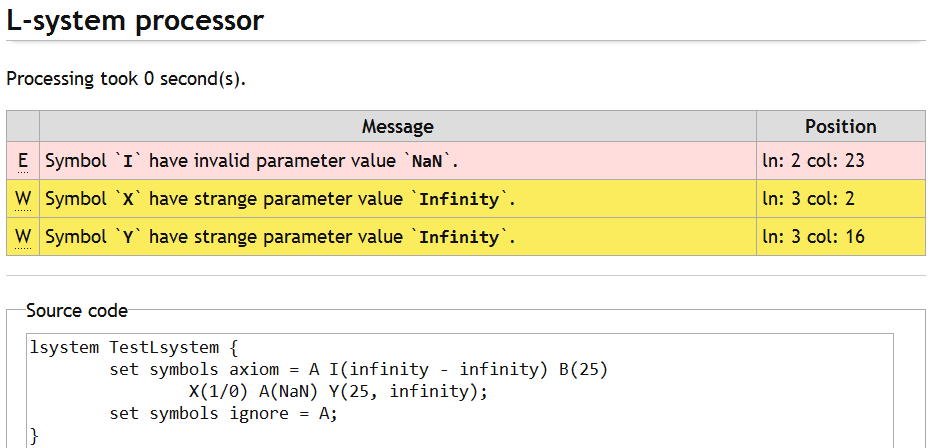
\includegraphics[width=0.9\linewidth]{FilterComponentMessages}}
	\caption{The result of processing }
	\label{fig:messagesFilter}
\end{figure}

\subsection{Usage in real process configuration}

New we can use the filter component in more complex process configuration.
We will alter actual \emph{SymbolPrinter} process configuration (see appendix \ref{sec:stdLibSymbolPrinter}) by extending  it with our filter component as shows \autoref{fig:lastFilterScheme}.

\begin{figure}[h!]
	\centering
	\begin{tikzpicture}[->,auto, node distance=33mm,>=latex,shorten >=2pt]
		\node (it) [block] {Iterator};
		\node (in) [block, above of=it, node distance=20mm] {Axiom provider};
		\node (rand) [block, below of=it, node distance=20mm] {Random generator provider};
		\node (rw) [block, left of=it] {Rewriter};
		\node (filt) [blockx, right of=it] {Symbol filter};
		\node (print) [block, right of=filt] {Symbol printer};
		\node (out) [coord, right of=print] {};
				
		\draw (rw) to[bend left=40] (it);
		\draw (it) to[bend left=40] (rw);
		\draw (in) -- (it);
		\draw (it) -- (rand);
		\draw (it) -- (filt);
		\draw (filt) -- (print);
		\draw (print) -- node {output} (out);
	\end{tikzpicture}
	\caption{Extended \emph{SymbolPrinter} process configuration with the filter component}
	\label{fig:lastFilterScheme}
\end{figure}

Processing of \autoref{lsys:lastFilter} will result in output \texttt{F(2) F(4) F(256) F(Infinity)} along with warning about parameter of symbol \texttt{F}.

\begin{Lsystem}[label=lsys:lastFilter,caption={Test of extended \emph{SymbolPrinter} process configuration with created filter component}]
configuration FilteredSymbolPrinter {
	component AxiomProvider typeof AxiomProvider;
	component RandGenProvider typeof RandomGeneratorProvider;
	@component Filter typeof SymbolFilter;@

	container Rewriter typeof IRewriter default SymbolRewriter;
	container Iterator typeof IIterator
		default MemoryBufferedIterator;
	container SymbolProcessor typeof ISymbolProcessor
		default SymbolsSaver;

	connect RandGenProvider to Iterator.RandomGeneratorProvider;
	connect AxiomProvider to Iterator.AxiomProvider;
	connect Iterator to Rewriter.SymbolProvider;
	connect Rewriter to Iterator.SymbolProvider;
	@connect Filter to Iterator.OutputProcessor;@
	@connect SymbolProcessor to Filter.Output;@
}

lsystem TestLsystem {
	set symbols axiom = X(2);
	set symbols ignore = X;
	set iterations = 4;
	rewrite X(n) to F(n) X((n ^ n));
}

process TestLsystem with FilteredSymbolPrinter;
\end{Lsystem}













